% (find-LATEX "2020-1-C3-taylor-2.tex")
% (defun c () (interactive) (find-LATEXsh "lualatex -record 2020-1-C3-taylor-2.tex" :end))
% (defun D () (interactive) (find-pdf-page      "~/LATEX/2020-1-C3-taylor-2.pdf"))
% (defun d () (interactive) (find-pdftools-page "~/LATEX/2020-1-C3-taylor-2.pdf"))
% (defun e () (interactive) (find-LATEX "2020-1-C3-taylor-2.tex"))
% (defun u () (interactive) (find-latex-upload-links "2020-1-C3-taylor-2"))
% (defun v () (interactive) (find-2a '(e) '(d)) (g))
% (find-pdf-page   "~/LATEX/2020-1-C3-taylor-2.pdf")
% (find-sh0 "cp -v  ~/LATEX/2020-1-C3-taylor-2.pdf /tmp/")
% (find-sh0 "cp -v  ~/LATEX/2020-1-C3-taylor-2.pdf /tmp/pen/")
%   file:///home/edrx/LATEX/2020-1-C3-taylor-2.pdf
%               file:///tmp/2020-1-C3-taylor-2.pdf
%           file:///tmp/pen/2020-1-C3-taylor-2.pdf
% http://angg.twu.net/LATEX/2020-1-C3-taylor-2.pdf
% (find-LATEX "2019.mk")

% «.sombrero»			(to "sombrero")
% «.sampaio»			(to "sampaio")
% «.derivacao-implicita»	(to "derivacao-implicita")
% «.exercicio-1»		(to "exercicio-1")
% «.exercicio-2»		(to "exercicio-2")
% «.exercicio-3»		(to "exercicio-3")
% «.exercicio-4»		(to "exercicio-4")

\documentclass[oneside,12pt]{article}
\usepackage[colorlinks,citecolor=DarkRed,urlcolor=DarkRed]{hyperref} % (find-es "tex" "hyperref")
\usepackage{amsmath}
\usepackage{amsfonts}
\usepackage{amssymb}
\usepackage{pict2e}
\usepackage[x11names,svgnames]{xcolor} % (find-es "tex" "xcolor")
%\usepackage{colorweb}                 % (find-es "tex" "colorweb")
%\usepackage{tikz}
%
% (find-dn6 "preamble6.lua" "preamble0")
%\usepackage{proof}   % For derivation trees ("%:" lines)
%\input diagxy        % For 2D diagrams ("%D" lines)
%\xyoption{curve}     % For the ".curve=" feature in 2D diagrams
%
\usepackage{edrx15}               % (find-LATEX "edrx15.sty")
\input edrxaccents.tex            % (find-LATEX "edrxaccents.tex")
\input edrxchars.tex              % (find-LATEX "edrxchars.tex")
\input edrxheadfoot.tex           % (find-LATEX "edrxheadfoot.tex")
\input edrxgac2.tex               % (find-LATEX "edrxgac2.tex")
%
%\usepackage[backend=biber,
%   style=alphabetic]{biblatex}            % (find-es "tex" "biber")
%\addbibresource{catsem-slides.bib}        % (find-LATEX "catsem-slides.bib")
%
% (find-es "tex" "geometry")
\usepackage[a6paper, landscape,
            top=1.5cm, bottom=.25cm, left=1cm, right=1cm, includefoot
           ]{geometry}
%
\begin{document}

\catcode`\^^J=10
\directlua{dofile "dednat6load.lua"}  % (find-LATEX "dednat6load.lua")

% «defs»  (to ".defs")
% (find-LATEX "edrx15.sty" "colors-2019")
\long\def\ColorRed   #1{{\color{Red1}#1}}
\long\def\ColorViolet#1{{\color{MagentaVioletLight}#1}}
\long\def\ColorViolet#1{{\color{Violet!50!black}#1}}
\long\def\ColorGreen #1{{\color{SpringDarkHard}#1}}
\long\def\ColorGreen #1{{\color{SpringGreenDark}#1}}
\long\def\ColorGreen #1{{\color{SpringGreen4}#1}}
\long\def\ColorGray  #1{{\color{GrayLight}#1}}
\long\def\ColorGray  #1{{\color{black!30!white}#1}}
\long\def\ColorBrown #1{{\color{Brown}#1}}
\long\def\ColorBrown #1{{\color{brown}#1}}

\long\def\ColorShort #1{{\color{SpringGreen4}#1}}
\long\def\ColorLong  #1{{\color{Red1}#1}}

\def\frown{\ensuremath{{=}{(}}}
\def\True {\mathbf{V}}
\def\False{\mathbf{F}}

\def\drafturl{http://angg.twu.net/LATEX/2020-1-C2.pdf}
\def\drafturl{http://angg.twu.net/2020.1-C2.html}
\def\draftfooter{\tiny \href{\drafturl}{\jobname{}} \ColorBrown{\shorttoday{} \hours}}


%  _____ _ _   _                               
% |_   _(_) |_| | ___   _ __   __ _  __ _  ___ 
%   | | | | __| |/ _ \ | '_ \ / _` |/ _` |/ _ \
%   | | | | |_| |  __/ | |_) | (_| | (_| |  __/
%   |_| |_|\__|_|\___| | .__/ \__,_|\__, |\___|
%                      |_|          |___/      
%
% «title»  (to ".title")
% (c3m201taylor2p 1 "title")
% (c3m201taylor2a   "title")

\thispagestyle{empty}

\begin{center}

\vspace*{1.2cm}

{\bf \Large Cálculo 3 - 2020.1}

\bsk

Aula 5 e 6: Aproximações de 1ª e 2ª ordem:

algumas aplicações

\bsk

Eduardo Ochs - RCN/PURO/UFF

\url{http://angg.twu.net/2020.1-C3.html}

\end{center}

\newpage

% «sombrero»  (to ".sombrero")
% (c3m201taylor2p 2 "sombrero")
% (c3m201taylor2    "sombrero")

{\bf Introdução}

\ssk

Daqui a algumas aulas nós vamos começar a estudar
\ColorRed{superfícies em $\R^3$}. Por exemplo, a superfície abaixo é o
conjunto:
%
$$S = \setofst{(x,y,x)}{r = \sqrt{x^2 + y^2}, z = \sen(r)/r}:$$
%
% (find-node "(octave)Three-Dimensional Plots" "sombrero")
% (find-fline "/usr/share/info/mesh.png")
% (find-fline "~/LATEX/2020-1-C3/")
% (find-latexgimp-links "2020-1-C3/mesh")
% (find-fline   "~/LATEX/2020-1-C3/mesh.png")
$$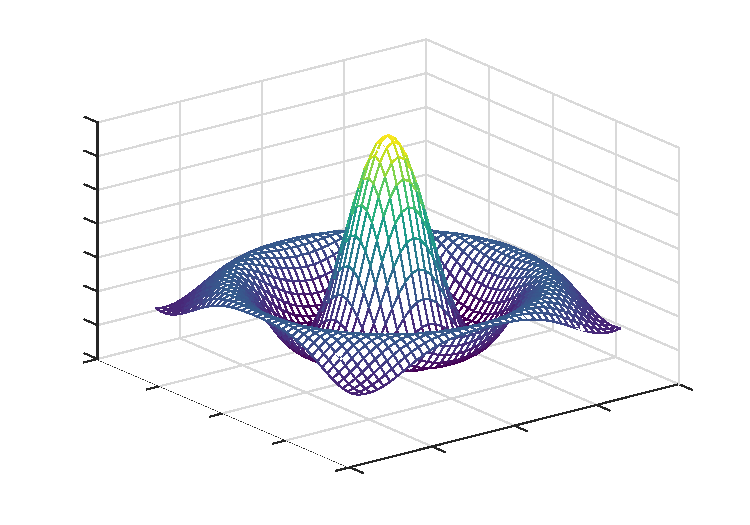
\includegraphics[height=5cm]{2020-1-C3/mesh.png}$$

\newpage

...e pra conseguir entender essa superfície e outras sem precisar
calcular centenas de pontos delas nós vamos ter que aprender estender
a idéia de aproximações de 1ª e 2ª ordem da aula anterior de vários
jeitos. Por exemplo:

\msk

1) vamos aprender a lidar com trajetórias $F:\R→\R^3$ em que todo
ponto $F(t)$ pertence ao conjunto $S$,

2) vamos aprender a fazer aproximações de 1ª ordem de $S$ que vão ser
\ColorRed{planos},

3) vamos aprender a fazer aproximações de 2ª ordem de $S$ que vão ser
\ColorRed{cônicas} com equações da forma $z=ax^2 + by^2 + cxy + dx +
ey +f$, que você deve ter visto no final do curso de Geometria
Analítica...

\msk

...mas pra isso vamos ter que rever \ColorRed{taxas relacionadas},
\ColorRed{derivação implícita} e \ColorRed{diferenciais}, e depois
adaptar as suas idéias para mais dimensões.


\newpage

% «sampaio»  (to ".sampaio")
% (c3m201taylor2p 4 "sampaio")
% (c3m201taylor2    "sampaio")

O João Carlos Vieira Sampaio, da UFSCar, tem um material muito bom em
Português sobre taxas relacionadas e diferenciais. Link:

\ssk

\url{https://www.dm.ufscar.br/profs/sampaio/calculo1\_aula14.pdf}

\ssk

Hoje vamos entender as idéias desse PDF até o exemplo 14.3 dele, mas
com mais ênfase em visualização -- vamos fazer alguns desenhos que ele
não faz, e vamos tentar visualizar todas as idéias ao invés de fazer
as contas que ele faz pra provar que essas idéias são verdade. Daqui a
pouco você vai fazer o curso de Cálculo Numérico do Fábio e você vai
fazer todas as contas horríveis lá!

\msk

\ColorRed{Comece lendo esse PDF até o exemplo 14.3. Anote suas dúvidas
  e compartilhe-as no Telegram. Daqui a pouco eu vou pôr mais
  instruções nestes slides -- que trechos do ``aula14.pdf'' é pra
  pular, que desenhos é pra fazer, e alguns exercícios extras.}



\newpage

% «derivacao-implicita»  (to ".derivacao-implicita")
% (c3m201taylor2p 5 "derivacao-implicita")
% (c3m201taylor2    "derivacao-implicita")
% «exercicio-1»  (to ".exercicio-1")
% (c3m201taylor2p 5 "exercicio-1")
% (c3m201taylor2    "exercicio-1")

% (find-sampaio14page 3 "derivando implicitamente")
% (find-sampaio14text 3 "derivando implicitamente")

{\bf Derivação implícita}

\ssk

No Exemplo 14.2 o João Carlos Sampaio usa derivação implícita supondo
que o leitor lembra bem de como derivar implicitamente... vamos fazer
uma mini-revisão disso usando o exemplo dele.

\msk


{\bf Exercício 1.}

Digamos que $g(x) = \sqrt{x^2 + f(x)}$. Calcule $g'(x)$. Chame de
[a]'' a equação ``$g'(x) = \ldots$'' que você obteve. Digamos que
$g'(x)=0$ em [a]. Chame esta nova equação, ``$0 = \ldots$'', de [b].
Digamos que não sabemos nem o valor de $f(x)$ nem o de $f'(x)$ em [b],
e vamos tratá-los como variáveis. Isole o $f'(x)$ em [b] e obtenha uma
equação da forma ``$f'(x) = \ldots$'', onde este ``$\ldots$'' pode
mencionar $f(x)$ mas não $f'(x)$. Chame esta nova equação de [c].

Diga quem são as equações [a], [b] e [c] arrumando as suas contas de
um jeito legível.


\newpage

% «exercicio-2»  (to ".exercicio-2")
% (c3m201taylor2p 6 "exercicio-2")
% (c3m201taylor2    "exercicio-2")

{\bf Exercício 2.}

\ssk

Digamos que $y=f(x)$ e $z=\sqrt{x^2 + y}$.

Aqui nós vamos traduzir o exercício anterior para a ``notação de
Leibniz'', que usa $\frac{dy}{dx}$ ao invés de $f'(x)$ e
$\frac{dz}{dx}$ ao invés de $g'(x)$.

Traduza para a notação de Leibniz a sua equação [a] do exercício
anterior e chame a versão traduzida de [a']. Faça o mesmo para as
equações [b] e [c], e chame as versões traduzidas delas de [b'] e [c'].

No final do exercício 1 você arrumou todas as suas contas de uma forma
legível. Faça o mesmo agora, mas com as versões traduzidas. No final
você deve obter um modo de calcular $\frac{dy}{dx}$ a partir de $x$ e
$y$.


\newpage

% «exercicio-3»  (to ".exercicio-3")
% (c3m201taylor2p 7 "exercicio-3")
% (c3m201taylor2    "exercicio-3")

{\bf Revisão (?) de diferenciais}

\ssk

A seção 14.2 da aula do João Carlos Sampaio é sobre
\ColorRed{diferenciais}, que a gente não costuma ver direito em
Cálculos 1 e 2. Leia ela.

\msk

Se escrevermos $f'(x)dx$ na notação de Leibniz obtemos
$\frac{dy}{dx}dx$, e a idéia de diferenciais é que vamos
\ColorRed{definir} $dy$ como sendo $dy := \frac{dy}{dx}dx$. Aí nós
vamos poder cortar os `$dx$'s em $\frac{dy}{dx}dx = dy$ -- mas isso só
vai funcionar porque definimos tudo do jeito certo \ColorRed{e porque
  vamos tratar o ``$dx$'' sozinho como uma nova variável}.

\msk

{\bf Exercício 3.} Multiplique os dois lados da sua equação [c'] por
$dx$ e faça o cancelamento $\frac{dy}{dx}dx \squigto dy$ onde for
possível. Obtenha uma equação da forma ``$dy = \ldots$'' em que esse
``$\ldots$'' só pode mencionar as variáveis $x$, $y$ e $dx$. Chame
esta nova equação de [c''].



\newpage

% «exercicio-4»  (to ".exercicio-4")
% (c3m201taylor2p 8 "exercicio-4")
% (c3m201taylor2    "exercicio-4")

{\bf Exercício 4.}

Multiplique os dois lados da sua equação [a'] por $dx$ e rearrume o
resultado pra obter uma equação da forma ``$dz = \ldots dx + \ldots
dy$'', onde as expressões ``$\ldots$'' só podem mencionar as variáveis
$x$ e $y$. Chame esta equação nova de [a''].





% https://www.dm.ufscar.br/profs/sampaio/calculo1_aula14.pdf
% (code-pdf-page "sampaio14" "$S/https/www.dm.ufscar.br/profs/sampaio/calculo1_aula14.pdf")
% (code-pdf-text "sampaio14" "$S/https/www.dm.ufscar.br/profs/sampaio/calculo1_aula14.pdf")
% (find-sampaio14page)
% (find-sampaio14text)
% (find-sampaio14page 3 "14.2      Diferenciais")
% (find-sampaio14text 3 "14.2      Diferenciais")







% (find-sh "locate -i isabel")
% (find-fline "/sda1/home/edrx/2019.1-C3/Ana_Isabel/")
% (c3q192  8 "20190823" "Parábolas parametrizadas em R2; aproxs de 1a e 2a ordem")
% (find-books "__analysis/__analysis.el" "apex-calculus")

% (c3m191)
% (c3m191p)
% (c3m192)
% (c3m192p)




%\printbibliography

\end{document}

%  __  __       _        
% |  \/  | __ _| | _____ 
% | |\/| |/ _` | |/ / _ \
% | |  | | (_| |   <  __/
% |_|  |_|\__,_|_|\_\___|
%                        
% <make>

 (eepitch-shell)  (eepitch-kill)  (eepitch-shell) # (find-LATEXfile
"2019planar-has-1.mk") make -f 2019.mk STEM=2020-1-C3-taylor-2
veryclean make -f 2019.mk STEM=2020-1-C3-taylor-2 pdf

% Local Variables:
% coding: utf-8-unix
% ee-tla: "c3m201taylor2"
% End:
